\documentclass[12pt]{article}

\usepackage{tabularx}
\usepackage[a4paper,margin=2.5cm, bottom=3.5cm]{geometry}
\usepackage{fancyhdr}
\usepackage{listings}
\usepackage{booktabs}
\usepackage{float}
\usepackage{subcaption}
\usepackage{graphicx}
\usepackage{amsmath}
\usepackage{amssymb}
\usepackage{amsthm}
\usepackage{array}
\usepackage[table]{xcolor}
\usepackage{pgfplots}
\usepackage{pgfplotstable}
\usepackage{multirow}
\usepackage{tikz}
\usepackage[hidelinks]{hyperref}
\usepackage{titling}
\pgfplotsset{compat=1.17}

\theoremstyle{definition}
\newtheorem*{example}{Example}
\setlength{\headheight}{40pt}
\setlength{\parindent}{0pt}
\setlength{\parskip}{1ex}
\renewcommand{\headrulewidth}{0pt}

\newcommand{\subfiguresize}{.3\textwidth}
\DeclareMathOperator*{\median}{median}

\newcommand{\biggerforall}{\mbox{\Large $\mathsurround0pt\forall$}} 
\newcommand{\bigforall}{\mbox{\large $\mathsurround0pt\forall$}} 
\newcommand{\biggerexists}{\mbox{\Large $\mathsurround0pt\exists$}} 
\newcommand{\bigexists}{\mbox{\large $\mathsurround0pt\exists$}} 

\lstset {
    basicstyle = \small\ttfamily,
    keywordstyle = \color{blue},
    commentstyle = \color{black!30},
    comment = [l]{//},
    morecomment = [s]{/*}{*/},
    identifierstyle=,
    keywords = {
        let,
        mut,
        for,
        in,
        if,
        else,
        continue,
        break,
        pub,
        struct,
        impl,
        type,
        Self,
        u8,u16,u32,u64,
        i8,i16,i32,i64,
        f32,f64,
        usize,
    }
}

\pagestyle{fancy}
\fancyhead{}
\fancyhead[L]{
    \renewcommand{\arraystretch}{1.5}
    \begin{tabularx}{\textwidth}{|X|X|}
        \hline
        \large \bf Image processing & \normalsize \thetitle \\
        \hline
    \end{tabularx}
}
\fancyfoot[C]{\thepage}

\renewcommand{\maketitle}{
    \thispagestyle{plain}
    \renewcommand{\arraystretch}{2}
    \begin{flushleft}
        \begin{tabularx}{0.95\textwidth}{|X|X|}
            \hline
            \bf \large Image Processing                   & \bf \large \thetitle                           \\ \hline
            \multicolumn{2}{|l|}{
                \textbf{Task variant:} Group 1
            }                                                                                               \\ \hline
            \textbf{Day and time:} Mon, 14:00             & \textbf{Full name:} \textsc{Jakub Pawlak}       \\
            \textbf{Academic year:} {2022/23} & \textbf{Full name:} \textsc{Magdalena Paku\l a} \\
            \hline
        \end{tabularx}
    \end{flushleft}
    \vspace{1em}
    \renewcommand{\arraystretch}{1}
}
\graphicspath{{img},{../img}}
\usepackage{listings}
\usetikzlibrary{matrix}
\tikzset{square matrix/.style={
    matrix of nodes,
    nodes in empty cells,
    column sep=-\pgflinewidth, row sep=-\pgflinewidth,
    nodes={draw,
      minimum height=#1,
      anchor=center,
      text width=#1,
      align=center,
      inner sep=0pt
    },
  },
  square matrix/.default=1.5em
}

\title{Task No.~3}

\begin{document}
\maketitle

\section{Description of the implementation of the basic \texorpdfstring{\\ }{} morphological operations}

\subsection*{Optimization}

To make operations on binary images more efficient,
we represent the binary mask not as an image or collection of coordinates,
but as a slice of memory where each bit corresponds to a specific pixel.
This is done to firstly reduce the memory size, and secondly to make the operations faster by enabling the use of
binary operators, which are $\mathcal{O}(1)$.

Since the mask is a finite cartesian coordinate plane, we can assign each point $(x,y)$,
a unique number $n = x + wy$, where $w$ is the width of the coordinate plane.
The pixel will be assigned the $n$-th bit.

Therefore, for a $3\times3$ mask, it will be represented in the following way

\begin{center}
    \begin{tikzpicture}[baseline=(Center.base)]
        \matrix[square matrix]
        {
        |[fill=gray]| & |[fill=gray]| & \\
        & |(Center)[fill=gray]| & \\
        & & |[fill=gray]| \\
        };
    \end{tikzpicture}
    $\; \Longleftrightarrow \; (100010011)_2$
\end{center}

\vfill

However, since the input is in the image form, we need a function to convert between the image and binary representations.
This function will take the image, as well as a set of $(x,y)$ coordinates, and construct the mask from the pixels neighboring $(x,y)$.

\begin{equation}
    \mathbf{M}(A,x,y) \to B
\end{equation}

\begin{center}
    \begin{tikzpicture}[baseline=(Center.base)]
        \matrix[square matrix]
        {
        |[fill=gray]|&&|[fill=gray]|&&|[fill=gray]|\\
        |[fill=gray]|&|[fill=gray]| & |[fill=gray]| && \\
        && |(Center)[fill=gray]|{$\bullet$} && \\
        && & |[fill=gray]| &|[fill=gray]| \\
        &|[fill=gray]|&|[fill=gray]|&&|[fill=gray]|\\
        };
    \end{tikzpicture}
    $\; \mapsto \; $
    \begin{tikzpicture}[baseline=(Center.base)]
        \matrix[square matrix]
        {
        |[fill=gray]| & |[fill=gray]| & \\
        & |(Center)[fill=gray]| & \\
        & & |[fill=gray]| \\
        };
    \end{tikzpicture}
\end{center}

\vfill
\pagebreak[2]

\begin{lstlisting}
pub fn from_image(image: &GrayImage, x: u32, y: u32) -> Mask {
    let mut mask = Mask::new();
    for i in 0..3 {
        for j in 0..3 {
            if is_unwritable(image, x, y, i, j) {
                continue;
            }
            mask.set_pixel(
                i, 
                j, 
                image.get_pixel(x + i - 1, y + j - 1)
            );
        }
    }
    mask
}
\end{lstlisting}

\vspace{2em}
We have also implemented the reverse function, 
to set the pixels in the image from the binary implementation.

\begin{lstlisting}
pub fn write_to_image(
    &self, 
    image: &mut GrayImage, 
    x: u32, 
    y: u32
) {
    for i in 0..3 {
        for j in 0..3 {
            if is_unwritable(image, x, y, i, j) {
                continue;
            }
            image.put_pixel(
                x + i - 1, 
                y + j - 1, 
                self.get_pixel(i, j)
            );
        }
    }
}
\end{lstlisting}

Note that this function, 
will overwrite the existing pixels if they are foreground in image, 
but background in mask.

\pagebreak[4]
\subsection{Dilation}

The dilation of a binary image $A$ by a binary mask $B$ is defined as
\begin{equation}
    A \oplus B = \bigcup_{a \in A} B_a
\end{equation}

\begin{center}
    \begin{tikzpicture}[baseline=(A.base)]
        \matrix[square matrix]
        {
        &&\\
        &|(A)[fill=gray]|&|[fill=gray]|\\
        |[fill=gray]|&|[fill=gray]|&\\
        };
    \end{tikzpicture}
    $\; \oplus \; $
    \begin{tikzpicture}[baseline=(A.base)]
        \matrix[square matrix]
        {
        & |[fill=gray]| & \\
        & |[fill=gray]|$\odot$ & \\
        & &  \\
        };
    \end{tikzpicture}
    $\; = \; $
    \begin{tikzpicture}[baseline=(A.base)]
        \matrix[square matrix]
        {
        &|[fill=gray]|&|[fill=gray]|\\
        |[fill=gray]|&|[fill=gray]|&|[fill=gray]|\\
        |[fill=gray]|&|[fill=gray]|&\\
        };
    \end{tikzpicture}
\end{center}

To calculate the dilation of image $A$ by mask $B$, 
we first need to allocate a new image $A'$.
This is done, because the dilation operating on more than one pixel, 
so we cannot corrupt the original data.

Then, for each pixel $(x,y) \in A$, if $A(x,y)$ is foreground,
we perform the folliwing steps:
\begin{enumerate}
    \item Convert the neighbourhood of $(x,y)$ from $A'$ to binary mask $B'$
    \item Apply the binary or operation to the acquired mask and the mask $B$
    \item Save the result to the image $A'$
\end{enumerate}

\begin{lstlisting}
for (x, y, pixel) in image.enumerate_pixels() {
    if !is_foreground(pixel) {
        continue;
    }
    let new_image_mask = Mask::from_image(&new_image, x, y);
    let mask = self.mask | new_image_mask;
    mask.write_to_image(&mut new_image, x, y);
}
\end{lstlisting}

\subsection{Erosion}

Erosion of $A$ by $B$ is defined as
\begin{equation}
    A \ominus B = \left\{ (x,y) \mid B_{(x,y)} \subseteq A \right\}
    \label{eq:erosion-formal-def}
\end{equation}

\begin{center}
    \begin{tikzpicture}[baseline=(A.base)]
        \matrix[square matrix]
        {
        &&|[fill=gray]|\\
        &|(A)[fill=gray]|&|[fill=gray]|\\
        |[fill=gray]|&|[fill=gray]|&\\
        };
    \end{tikzpicture}
    $\; \ominus \; $
    \begin{tikzpicture}[baseline=(A.base)]
        \matrix[square matrix]
        {
        & |[fill=gray]| & \\
        & |[fill=gray]|$\odot$ & \\
        & &  \\
        };
    \end{tikzpicture}
    $\; = \; $
    \begin{tikzpicture}[baseline=(A.base)]
        \matrix[square matrix]
        {
        &&\\
        &&|[fill=gray]|\\
        &|[fill=gray]|&\\
        };
    \end{tikzpicture}
\end{center}

We can check the condition that $B_{(x,y)} \subseteq A$ very easily by usin the binary and operation.
\begin{equation}
    B_{(x,y)} \subseteq A \;\Leftrightarrow\; B = \left( B \land \mathbf{M}(A,x,y) \right)
\end{equation}

\pagebreak[2]
We can thus rewrite eq. (\ref{eq:erosion-formal-def}) as:
\begin{equation}
    A \ominus B = \left\{ (x,y) \mid B = \big( B \land \mathbf{M}(A,x,y) \big) \right\}
\end{equation}


Therefore, to calculate $A \ominus B$, for each $(x,y) \in A$, we perform the following steps:
\begin{enumerate}
    \item Convert the neighbourhood of $(x,y)$ from $A$ to binary form
    \item Apply the binary and operation to the acquired mask and the mask $B$
    \item If the result of the prevous step is equal to $B$, we set $A'(x,y)$ to foreground
\end{enumerate}

\pagebreak[3]
\begin{lstlisting}
for (x, y, pixel) in image.enumerate_pixels() {
    let mask = self.mask & Mask::from_image(&image, x, y);
    if mask == self.mask {
        new_image.put_pixel(x, y, FOREGROUND_PIXEL);
    }
}
\end{lstlisting}

\subsection{Opening}

\subsection{Closing}

\subsection{Hit-or-miss transform}

The HMT of $A$ with $\mathbf{B}$ where $\mathbf{B} = (B_1,B_2)$, is defined as
\begin{equation}
    A \otimes \mathbf{B} = \left\{ p \mid \biggerforall\limits_{\substack{b_1 \in B_1 \\ b_2 \in B_2}}\; p + b_1 \in A \land p + b_2 \notin A  \right\}
\end{equation}

\begin{center}
    \begin{tikzpicture}[baseline=(A.base)]
        \matrix[square matrix]
        {
        &&|[fill=gray]|&&\\
        &|[fill=gray]|&&|[fill=gray]|&\\
        &|[fill=gray]|&|(A)[fill=gray]|&|[fill=gray]|&\\
        &|[fill=gray]|&&|[fill=gray]|&\\
        &&&&\\
        };
    \end{tikzpicture}
    $\; \ominus \; $
    \begin{tikzpicture}[baseline=(A.base)]
        \matrix[square matrix]
        {
        & |[fill=green]| & \\
        & $\odot$ & |[fill=red]| \\
        & &|[fill=red]|  \\
        };
    \end{tikzpicture}
    $\; = \; $
    \begin{tikzpicture}[baseline=(A.base)]
        \matrix[square matrix]
        {
        &&&&\\
        &&&&\\
        &&&|[fill=gray]|&\\
        &|[fill=gray]|&&|[fill=gray]|&\\
        &|[fill=gray]|&&|[fill=gray]|&\\
        };
    \end{tikzpicture}
\end{center}

However, for our implementation, we will use the following property:
\begin{equation}
    A \circledast \mathbf{B} = (A \ominus B_1) \cap (A^C \ominus B_2)
\end{equation}

Which we can rewrite to make use of the binary operators as the following:

\begin{equation}
    A \circledast \mathbf{B} = \left\{ (x,y) \mid
    \Big(B_1 = \big(B_1 \land \mathbf{M}(A,x,y)\big)\Big)
    \land \Big( B_2 = \big( B_2 \land \neg \mathbf{M}(A,x,y) \big) \Big)
    \right\}
\end{equation}

\section{Analysis of the results of the basic morphological operations}

\section{Description of the implementation of the assigned variant of morphological algorithm}

\subsection{Description}
The algorithm we had to implement is the convex hull.

It is used to eliminate any concavities from the shape.
The calculation of a convex hull of some image $A$ works as follows:

\begin{enumerate}
    \item For each structuring element $\mathbf{B}^i$ shown on fig. \ref{fig:convex-hull-kernels}:
    \begin{enumerate}
        \item We start with $X^i_0 = A$
        \item We repeatedly calculate $X^i_k = (X^i_{k-1} \otimes \mathbf{B}^i) \cup A$
        \item When $X^i_k = X^i_{k-1}$, we return $D^i = X^i_k$
    \end{enumerate}
    \item The final result is union of all $D^i$
\end{enumerate}

\begin{figure}[H]\centering
    \begin{subfigure}[t]{.2\textwidth}\centering
        \begin{tikzpicture}
            \matrix[square matrix]
            {
            |[fill=green]|&&\\
            |[fill=green]|&|[fill=red]|$\odot$&\\
            |[fill=green]|&&\\
            };
        \end{tikzpicture}
        \caption{$\mathbf{B}^1$}
        \label{kernel-convex-left}
    \end{subfigure}
    \begin{subfigure}[t]{.2\textwidth}\centering
        \begin{tikzpicture}
            \matrix[square matrix]
            {
            |[fill=green]|&|[fill=green]|&|[fill=green]|\\
            &|[fill=red]|$\odot$&\\
            &&\\
            };
        \end{tikzpicture}
        \caption{$\mathbf{B}^2$}
        \label{kernel-convex-up}
    \end{subfigure}
    \begin{subfigure}[t]{.2\textwidth}\centering
        \begin{tikzpicture}
            \matrix[square matrix]
            {
            &&|[fill=green]|\\
            &|[fill=red]|$\odot$&|[fill=green]|\\
            &&|[fill=green]|\\
            };
        \end{tikzpicture}
        \caption{$\mathbf{B}^3$}
        \label{kernel-convex-right}
    \end{subfigure}
    \begin{subfigure}[t]{.2\textwidth}\centering
        \begin{tikzpicture}
            \matrix[square matrix]
            {
            &&\\
            &|[fill=red]|$\odot$&\\
            |[fill=green]|&|[fill=green]|&|[fill=green]|\\
            };
        \end{tikzpicture}
        \caption{$\mathbf{B}^4$}
        \label{kernel-convex-down}
    \end{subfigure}
    \caption{Structuring elements used for convex hull}
    \label{fig:convex-hull-kernels}
\end{figure}

\pagebreak[2]
\subsection{Implementation}

The implementation can be split into 2 distinct parts.
The first one is calculating $D^i$ for a given $B^i$.
We will refer to this step as ``saturating'' the image with the hit-or-miss transformation.
The second step is merging all of the resulting images into one.



\section{Analysis of the results of the assigned variant of morphological algorithm}

\begin{figure}[H]\centering
    \begin{subfigure}[t]{\subfiguresize}
        \includegraphics[width=\textwidth]{img/image1.png}
        \caption{before}
    \end{subfigure}
    \hspace{2em}
    \begin{subfigure}[t]{\subfiguresize}
        \includegraphics[width=\textwidth]{img/image1-convexhull.png}
        \caption{after}
    \end{subfigure}\\[2em]

    \begin{subfigure}[t]{\subfiguresize}
        \includegraphics[width=\textwidth]{img/image2.png}
        \caption{before}
    \end{subfigure}
    \hspace{2em}
    \begin{subfigure}[t]{\subfiguresize}
        \includegraphics[width=\textwidth]{img/image2-convexhull.png}
        \caption{after}
    \end{subfigure}
    \caption{Result of applying the convex hull}
\end{figure}

\section{Description of the implementation of the assigned segmentation variant}
\subsection{Description}
Region growing is a simple region-based image segmentation method that involves starting from a seed point in the image and expanding the region to include neighboring pixels that have similar characteristics to the seed point. 
Our implementation uses a breadth-first search algorithm to expand the region from the seed point. It maintains a queue of pixels to visit and adds the neighboring pixels of each pixel to the queue if they have a similar intensity value to the seed point, within a specified tolerance. The resulting image is a binary image with the region of interest marked in white and the rest of the image marked in black.

\subsection{Implementation}

In our implementation, $seed_x$ and $seed_y$ represent the x and y coordinates, respectively, of the seed point in the image chosen by the user. The seed point is also the starting point for the region growing algorithm. The $tolerance$ is also chosen by the user. Therefore, the 'RegionGrowing' struct was implement by declaring all of these three fields. Firstly, we are checking whether the chosen pixel is within the dimensions of the input image. If the seed point is within the image dimensions, the transformation for region growing can be performed.  Below the implementation of the 'Transformation' for 'Region Growing':

\begin{lstlisting}
impl Transformation for RegionGrowing {
    fn apply(&self, image: &mut image::ImageBuffer<Rgb<u8>, Vec<u8>>) {
        let mut new_image: GrayImage = ImageBuffer::new(image.width(), image.height());
        let mut queue = VecDeque::new();
        queue.push_back((self.seed_x, self.seed_y));
        let seed_pixel = image.get_pixel(self.seed_x, self.seed_y);
        while let Some((x, y)) = queue.pop_front() {
            if x >= image.width() || y >= image.height() {
                continue;
            }
            let pixel = image.get_pixel(x as u32, y as u32);
            let new_image_pixel = new_image.get_pixel(x as u32, y as u32);
            if new_image_pixel[0] == 0 && is_similar(pixel, seed_pixel , self.tolerance) {
                new_image.put_pixel(x as u32, y as u32, Luma([255]));
                queue.push_back((x + 1, y));
                queue.push_back((x, y + 1));
                queue.push_back((x - 1, y));
                queue.push_back((x, y - 1));
            }
        }
        //*image = new_image;
    }
}
\end{lstlisting}
The 'is_similar' function was implemented by taking in a reference to a pixel of type Rgb<u8> and a reference to a seed pixel of the same type, as well as a tolerance value of type u8. It calculates the difference between the value of the pixel and the seed pixel and returns true if the difference is less than or equal to the tolerance value. Below the implementation of the 'is_similar' function:
\begin{lstlisting}
fn is_similar(pixel: &Rgb<u8>, seed_pixel: &Rgb<u8>, tolerance: u8) -> bool {
    (pixel[0] as i32 - seed_pixel[0] as i32) <= tolerance as i32
}

\end{lstlisting}
\section{Analysis of the results of the assigned segmentation variant}
\section{Description of other changes which took place in the application}

Your GUI ? <3

\end{document}